\section{\label{sec:convention}Conventions for representing space groups}

\subsection{Conventional cell}

% Primitive basis and primitive cell
It is natural to choose a basis for a translation lattice of a space group such that all symmetry operations are represented by integer matrices.
Such a basis is called a \term{primitive basis} of the lattice, and a unit cell spanned by the primitive basis is called a \term{primitive cell}.

% Centered basis and conventional cell
Although the primitive basis is useful for mathematical and algorithmic treatments, we often use a non-primitive basis, called a \term{centered basis}, to represent the lattice for humans.
There are conventions on which centered basis to choose for each lattice system, which is called a \term{conventional basis} \cite{burzlaff2016crystal}.
A unit cell spanned by the conventional basis is called a \term{conventional cell}.
The conventional bases are chosen as right-handed with the following rules:

\paragraph{Triclinic lattice system ($aP$)}
Choose the Niggli reduced basis \cite{Krivy:a12875}.

\paragraph{Monoclinic lattice system ($mP, mS$)}
The only symmetry direction is labeled $\bm{b}$.
The other basis vectors $\bm{a}$ and $\bm{c}$ are chosen to be the shortest two vectors perpendicular to $\bm{b}$ with a non-acute angle.
The other settings to choose $\bm{a}$ or $\bm{c}$ as the unique axis are also used.

\paragraph{Orthorhombic lattice system ($oP, oS, oF, oI$)}
Choose basis vectors along the three twofold axes.

\paragraph{Tetragonal lattice system ($tP, tI$)}
The vector $\bm{c}$ is along the fourfold axis.
The $\bm{a}$ and $\bm{c}$ are chosen along the twofold axes perpendicular to each other.

\paragraph{Rhombohedral lattice system ($hR$)}
There are two descriptions in ITA~\cite{ITA2016}, \term{hexagonal axes} and \term{rhombohedral axes}.
For the hexagonal axes, the vector $\bm{c}$ is parallel to the threefold axis;
The $\bm{a}$ and $\bm{b}$ are chosen along twofold axes perpendicular to $\bm{c}$ with angle of $120^{\circ}$ so that lattice points occur at $2/3, 1/3, 1/3$ and $1/3, 2/3, 2/3$ (\term{obverse} setting).
The \term{reverse} setting with lattice points $1/3, 2/3, 1/3$ and $2/3, 1/3, 2/3$ is not used.
For the rhombohedral axes, choose the shortest three lattice vectors equivalent to the threefold axis.
See Fig~\ref{fig:hexagonal_axes} for the projections along $c$ of rhombohedral and hexagonal axes.

\begin{figure}[htb]
  \centering
  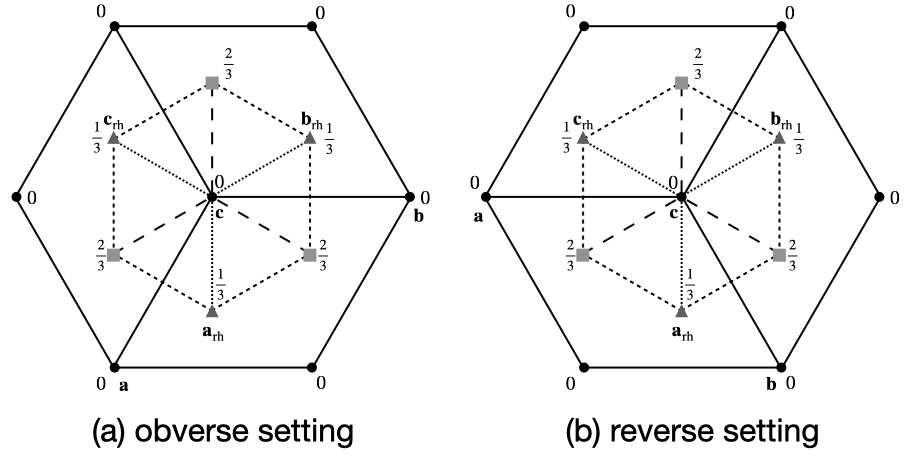
\includegraphics[width=0.9\textwidth]{figure/fig_hexagonal_axes.png}
  \caption{Projections of hexagonal axes of rhombohedral lattice in (a) obverse and (b) reserve settings.}
  \label{fig:hexagonal_axes}
\end{figure}

\paragraph{Hexagonal lattice system ($hP$)}
The vector $\bm{c}$ is parallel to the sixfold axis.
The $\bm{a}$ and $\bm{b}$ are chosen along twofold axes perpendicular to $\bm{c}$ with angle of $120^{\circ}$.

\paragraph{Cubic lattice system ($cP, cF, cI$)}
Choose basis vectors parallel to the fourfold axes.

\subsection{Hermann--Mauguin symbol}

The Hermann--Mauguin (HM) symbols represent space groups concisely.
The first constituent of the HM symbol characterizes the conventional cell of the translation lattice, one of $P, A, B, C, F, I$, and $R$.
The remained constituents describe generators of the space group.

One way to read the HM symbols is as follows (along with the example $Cmc2_{1}$):
\begin{enumerate}
  \item Read the conventional cell from the first constituent (base-centered basis $C$)
  \item Determine the geometric crystal class by ignoring translation parts ($mm2$)
  \item Determine the crystal class ($mm2 \, \rightarrow \, \mbox{orthorhombic}$)
  \item Read symmetry directions from Table~\ref{tab:hermann-mauguin}
\end{enumerate}

\begin{table}[htb]
  \caption{Symmetry directions for the short Hermann--Mauguin symbols in space groups}
  \label{tab:hermann-mauguin}
  \centering
  \begin{tabular}{cccc}
    \hline\hline
    Crystal system & Primary & Secondary & Tertiary  \\ \hline
    Triclinic                         & None  & & \\
    Monoclinic (unique axis $\bm{b}$) & [010] & & \\
    Orthorhombic                      & [100] & [010] & [001] \\
    Tetragonal                        & [001] & $\langle 100 \rangle$ & $\langle 1\overline{1}0 \rangle $ \\
    Trigonal ($P$ lattice) & [001] & $\langle 100 \rangle$ & None \\
                           & [001] & None & $\langle 1\overline{1}0 \rangle $ \\
    Trigonal ($R$ lattice, hexagonal axes) &
      $[001]_{\mathrm{hex}}$ & $\langle 100 \rangle_{\mathrm{hex}}$ & \\
    Trigonal ($R$ lattice, rhombohedral axes) &
      $[111]_{\mathrm{rhomb}}$ & $\langle 1\overline{1}0 \rangle_{\mathrm{rhomb}}$ & \\
    Hexagonal                        & [001] & $\langle 100 \rangle$ & $\langle 1\overline{1}0 \rangle$ \\
    Cubic                            & $\langle 001 \rangle$ & $\langle 111 \rangle$ & $\langle 1\overline{1}0 \rangle$ \\
    \hline\hline
  \end{tabular}
\end{table}

% The number of generators of space groups can be chosen as at most three.

\subsection{Conventional descriptions of space group types in ITA}

\subsubsection{Axis setting and cell choice for monoclinic crystal system}

(ITA-2.1.3.15)

\todo{Fix unique axes}

Axis settings for monoclinic systems are shown in Table~\ref{table-monoclinic-settings}.
Cell choices for monoclinic systems are shown in Table~\ref{table-monoclinic-cellchoice} and Fig.~\ref{fig:monoclinic-choices}.

\begin{table}[htb]
  \centering
  \small
  \caption{settings of monoclinic system}
  \label{table-monoclinic-settings}
  \begin{tabular}{c|cccccc}
    \hline\hline
    unique axis & $\mathbf{b}$ & $-\mathbf{b}$ & $\mathbf{c}$ & $-\mathbf{c}$ & $\mathbf{a}$ & $-\mathbf{a}$ \\
    setting & $\mathbf{a\underline{b}c}$ & $\mathbf{c\underline{\overline{b}}a}$ & $\mathbf{ab\underline{c}}$ & $\mathbf{ba\underline{\overline{c}}}$ & $\mathbf{\underline{a}bc}$ & $\mathbf{\underline{\overline{a}}bc}$ \\
    \hline
    \begin{tabular}{c}
    transformation \\ to $\mathbf{a\underline{b}c}$
    \end{tabular} &
      $\begin{pmatrix} 1& 0&0 \\ 0& 1&0 \\ 0& 0&1 \end{pmatrix}$ &
      $\begin{pmatrix}0& 0&1 \\0& -1&0 \\1& 0&0\end{pmatrix}$ &
      $\begin{pmatrix}0& 0&1 \\1& 0&0 \\0& 1&0\end{pmatrix}$ &
      $\begin{pmatrix} 1&0&0 \\ 0&0&1 \\ 0&-1&0 \end{pmatrix}$ &
      $\begin{pmatrix} 0&1&0 \\ 0&0&1 \\ 1&0&0 \end{pmatrix}$ &
      $\begin{pmatrix} 0&-1&0 \\ 1&0&0 \\ 0&0&1 \end{pmatrix}$ \\
    \hline
    Cell choice 1 & $C \to C$ & $A \to C$ & $A \to C$ & $B \to C$ & $B \to C$ & $C \to C$ \\
    Cell choice 2 & $A \to A$ & $C \to A$ & $B \to A$ & $A \to A$ & $C \to A$ & $B \to A$ \\
    Cell choice 3 & $I \to I$ & $I \to I$ & $I \to I$ & $I \to I$ & $I \to I$ & $I \to I$ \\
    \hline\hline
  \end{tabular}
\end{table}

\begin{table}[htb]
  \centering
  \caption{transformation of cell choices in monoclinic system}
  \label{table-monoclinic-cellchoice}
  \begin{tabular}{c|ccc}
    \hline\hline
    choice                 & $b1$                                                & $b2$                                                  & $b3$                                                  \\
    \hline
    transformation to $b1$ & $\begin{pmatrix} 1&0&0\\0&1&0\\0&0&1 \end{pmatrix}$ & $\begin{pmatrix} -1&0&1\\0&1&0\\-1&0&0 \end{pmatrix}$ & $\begin{pmatrix} 0&0&-1\\0&1&0\\1&0&-1 \end{pmatrix}$ \\
    \hline
    centering              & $C \to C$                                           & $A \to C$                                             & $I \to C$                                             \\
    \hline\hline
  \end{tabular}
\end{table}

\begin{figure}[htb]
  \centering
  \includegraphics[width=10cm]{figure/monoclinic_choices.eps}
  \caption{choices of monoclinic system}
  \label{fig:monoclinic-choices}
\end{figure}

\subsubsection{Axis setting for orthorhombic crystal system}

Axis settings for orthorhombic systems are shown in Table~\ref{table-orthorhombic-settings}.

\begin{table}[htb]
  \centering
  \small
  \caption{settings of orthorhombic system}
  \label{table-orthorhombic-settings}
  \begin{tabular}{c|cccccc}
    \hline\hline
    settings & $\mathbf{abc}$ & $\mathbf{ba\overline{c}}$ & $\mathbf{cab}$ & $\mathbf{\overline{c}ba}$ & $\mathbf{bca}$ & $\mathbf{a\overline{c}b}$ \\
    \hline\hline
    \begin{tabular}{c}
    transformation \\ to $\mathbf{abc}$
    \end{tabular} &
      $\begin{pmatrix} 1& 0&0 \\ 0& 1&0 \\ 0& 0&1 \end{pmatrix}$ &
      $\begin{pmatrix} 0&1&0 \\ 1&0&0 \\ 0&0&-1 \end{pmatrix}$ &
      $\begin{pmatrix}0& 0&1 \\1& 0&0 \\0& 1&0\end{pmatrix}$ &
      $\begin{pmatrix} 0&0&-1 \\ 0&1&0 \\ 1&0&0 \end{pmatrix}$ &
      $\begin{pmatrix} 0&1&0 \\ 0&0&1 \\ 1&0&0 \end{pmatrix}$ &
      $\begin{pmatrix} 1&0&0 \\ 0&0&-1 \\ 0&1&0 \end{pmatrix}$ \\
    \hline
    centering & $A \to A$ & $A \to B$ & $A \to C$ & $A \to C$ & $A \to B$ & $A \to A$ \\
              & $B \to B$ & $B \to A$ & $B \to A$ & $B \to B$ & $B \to C$ & $B \to C$ \\
              & $C \to C$ & $C \to C$ & $C \to B$ & $C \to A$ & $C \to A$ & $C \to B$ \\
    \hline\hline
  \end{tabular}
\end{table}

\subsubsection{Origin choice for centrosymmetric groups}

\subsubsection{Hexagonal axes}

\subsubsection{Standard ITA setting}

% Space-group type and setting: https://www.cryst.ehu.es/cgi-bin/cryst/programs/nph-def-choice
The standard ITA setting is one of the conventional descriptions for each space-group type used in the \textit{International Tables for Crystallography Vol. A} \cite{ITA2016}: unique axis b setting, cell choice 1 for monoclinic groups, hexagonal axes for rhombohedral groups, and origin choice 2 for centrosymmetric groups.


\subsection{Hall symbol}

Computer adapted symbol
